\chapter{Status quo and solution}
This section is an introduction into problem how the proposed solution looks like and what practices are used in the SwimmPair web application. 
\section{Problem description}
\par
A friend of mine reached out to me to ask me in order to ask if I could automate part of his agenda work agenda. Administration of swimming competitions and creating statistics is very repetitive and error-prone list of tasks. However, almost all the tasks from about organization are executed in the same order.
\par
The Czech Swimming Federation \footnote{https://www.czechswimming.cz} structure has to be modeled as objects in the application and database records as a storage. Thus, logical structure should be set and implemented in following order. Swimming referees belong to clubs, clubs are located in geographical regions. Swimming cup is organised by a club. Each Club contains several swimming referees and one of them is a club manager. When a Cup is online each Swimming referee can sign himself or herself up as available for the Cup. Club manager can also sign members of his club for a cup. At the end of the day, organizer of the cup assigns available referees that signed up to positions that he finds them suitable for. My friend, the chairman of referee committee should be able to perform additional administrative other tasks, such as adding and removing users, creating new clubs and modifying whole structure. Administrator can notify all visitors by posting an information psa on homepage.
\par
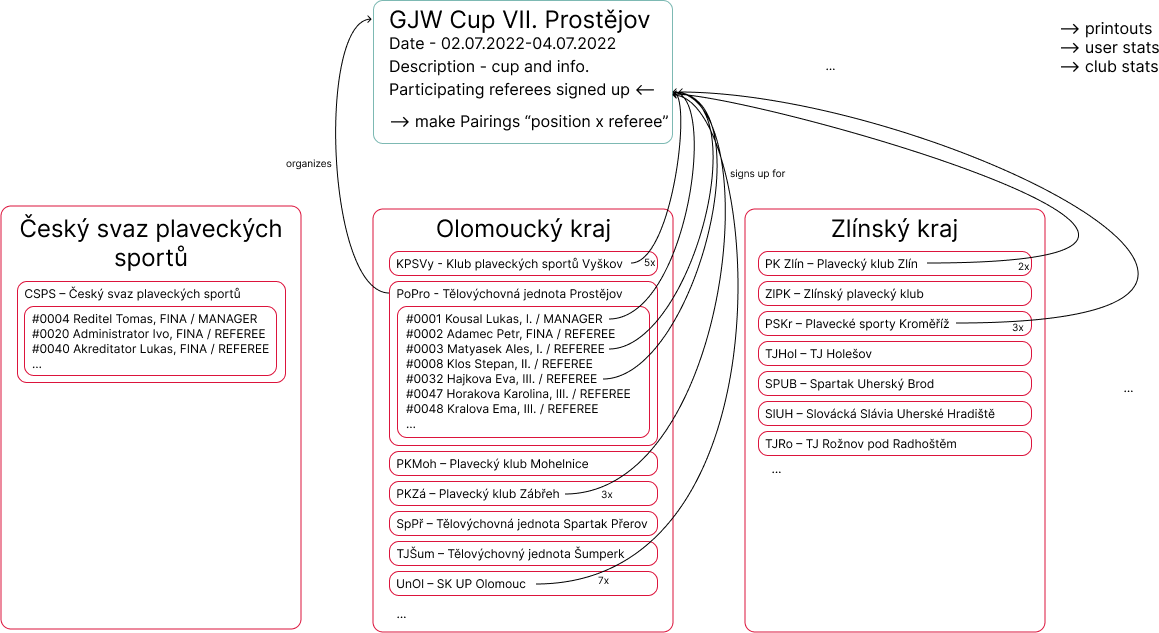
\includegraphics[scale=0.335]{img/swimmpair_schema.png}
\par
The SwimmPair system should deliver public listing of \textbf{users}, \textbf{cups}, \textbf{news}, \textbf{individual statistics} and \textbf{club statistics}. System should allow to browse stats on a yearly basis. This schema will then be appropriately modeled by objects and the schema will be shown below. 
\newpage
%%%An~example citation: %\cite{Andel07}
\section{Scenarios of storyboards}
These are tasks that have to be performed:
\begin{itemize}
    \item create swimming cup,
    \item perform pairing for swimming cup,
    \item manage swimming club,
    \item preview cup + print pairing,
    \item participate in cup or participate with teammates,
    \item statistics prereviews for accreditations renewal,
    \item statistics of referees,
    \item statistics of clubs,
    \item referees managment,
    \item clubs managment,
    \item clubs overview.
  \end{itemize}
\section{Model proposition}

\par
\subsection*{Cup}
Cup is the most important object of SwimmPair. A swimming Cup contains name, description, date and is affiliated to organising Club. Cup serves two purposes. Firstly - assigning referees for specific tasks (time tracking, computer support, head of the cup) has to be ready by the time the event takes place. Secondly - statistics summing up participations for Users and Clubs have to be calculated for each year over all cups in this time period. We also have to discriminate between upcoming and already past cups. Upcoming cups are displayed on the top, past cups should reside in the archive to be revisited for statistics purposes.
\subsection*{User}
\par
User is an entity modelling swimming referee. A referee participating in this system falls in one of three categories. These categories or levels if you wish are \textbf{referee}, \textbf{club manager} and \textbf{administrator}. User must be uniquely identifiable. A person i.e. User in the system is going to have profile information such as first name, family name, email address. Good practice of using an email address as a login information is going to be used here. User must also contain SwimmPair hierarchy listed above and indicator of one's skill and knowledge in the swimming field, i.e. referee category. User must also belong to exactly one club in our system.
\subsection*{Club}
\par
Club is an administrative unit of people. Club has specific name, abbrevation and ID in Czech Referee Federation. An image can be included as well. A club will be serving as a formal authority organising Cup - by a User who is Club Manager. Club is unanimously affiliated to Region. Statistics regarding performance of members of Club at swimming competitions must be implemented. Statistics have informative characted and will save time in the current status quo - keeping track of presence and work descriptions in Excel spreadsheets. 
%\subsection*{Post}
%%\par
Post is an informative snippet to be displayed at homepage to notify other swimmers about new event or anything worth paying attention to. Homepage should display last 3 posts and should be allowed to load more.
\subsection*{Region}
One of the 13 regions of the Czech Republic in which this system is used. Clubs are located in one of these regions. When new Club starts using SwimmPair, new region has to be added and potential clubs created and attached to this Region. 
We list objects of our application model and describe their properties and purpose.

\subsection*{Schema mockup}
Majority of focus should be on tables \textbf{users} and \textbf{cups} in presented schema. Users belong to clubs that belong to regions. These two entities \textbf{user} and \textbf{cups} are then brought together into table \textbf{availability} which lists referees for specific cups. Availabile users for cup are then paired in \textbf{pairing} where each couple can be assigned a position from \textbf{positions}.
\newline
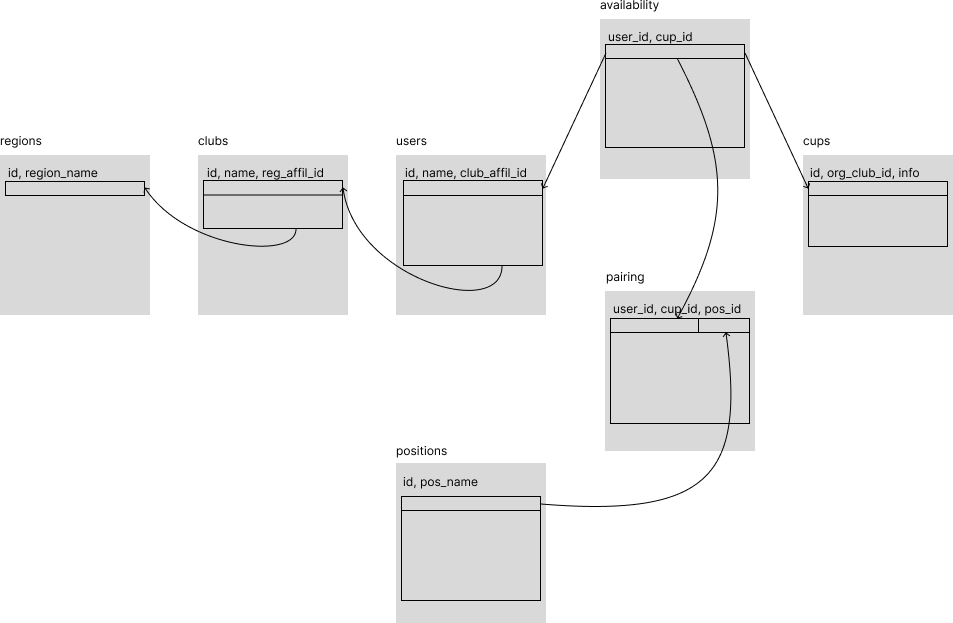
\includegraphics[scale=0.430]{img/swimmpair_db_mockup.png}
\subsection*{Availability}
Takes track of \textbf{User} available for \textbf{Cup} who are signed either by their team manager or themselves.
\subsection*{Pairing}
Record from availability is then taken and one or more \textbf{positions} are assigned to it. 
\subsection*{Position}
Predefined list of tasks necessary to be done at each cup. This list is probably never going to change since there is a fixed set of roles. Referees are going to be assigned to these positions for each cup by drag'n'drop user interface.
\newpage
\section{Frontend practices}
Several good practices have to be implemented to make SwimmPair easy to use. These practices are either well known or situation specific but they have one thing in common - they make the application good to use.
\subsection*{Smooth frontend browsing}
\par
Frontend of SwimmPair should be easy to use. There are several options and use cases of JavaScript that can come in handy. Reduction of page reloads is definitely a good way to go. Therefore there are going to be asynchronous JavaScript calls for obtain semi-partial data. After, next function will modify the DOM based on data received from asynchronous call. 
\subsection*{Multiple device types}
\par
Today is certain that there are users who want to browse our system from pc, tablet or smartphone and responsive design is a necessity. Since CSS3 supports media queries we are going to use them for creation of device specific styling.
\subsection*{Assigning referees to positions via. drag'n'drop}
\par
Assigning referees to positions for cups should be implemented via drag'n'drop. Dragging a referee, moving referee over the region specified for the positions and releasing mouse button. Double clicking this person is a good way of removing it.
\subsection*{Printouts of pairing}
Upcoming Cup can be directly printed from website and hanged as data printout. 
%\subsection*{Mobile administration}
%Since some things could be done from phone, a phone app without a necessity of web browser will have more native feel. Assigning by drag and drop would be very %hazardeous to do with regards to difference between mouse and finger. Also we are not certain that the Events are the same. Therefore full version %adminsitrative app should be necessary to be provided.
\subsection*{Appropriate design}
\par
Red blue and grey are colors that appear pretty much at a swimming pools. These colors will be used in our system as well. The elements should have fresh lightweave look and not appear heavy.
